\documentclass[10pt,a4paper, twocolumn]{report}
\usepackage[T1]{fontenc} 
\usepackage[utf8]{inputenc} 
\usepackage[spanish]{babel}
\usepackage{amsmath}
\usepackage{amsfonts}
\usepackage{amssymb}
\usepackage{graphicx}
\author{Antonio Molina García-Retamero}
\title{Optimización de redes neuronales mediante métodos bioinspirados}
\makeindex
\begin{document}
\onecolumn
\maketitle
\pagebreak
\tableofcontents
\pagebreak
\twocolumn

\chapter{Introduction}
\section{Notas}
\begin{itemize}
	\item En Haykin, en el capítulo 10, habla de los modelos teóricos de información. Hay cosas chulas, con las que puedo apoyar la metaplasticidad
	 \item Además, en ese mismo capítulo, trata también de las gausianas sus propiedades. También la relación con la entropía del conocimiento a priori de los parámetros de la gausiana.
	 \item Entre las diferentes técnicas de entrenamiento de redes RBF, la técnica de las k-medias puede ser sustituida por otras con tal de evitar el tiempo de cómputo. Sin embargo, a partir de estas k-medias podemos acelerar el proceso de aprendizaje en el BP. Tal vez así conseguimos mejores resultado en tiempo similares.
\end{itemize}

\section{La metaplasticidad en redes biológicas}

\section{Metaplasticidad en redes neuronales artificiales}
\section{Trabajos previos}
El término metaplasticidad aplicado a redes artificiales fué acuñado por el doctor Andina en (ref). Andina definió la metaplasticidad en redes neuronales artificales como:
\begin{quote}
During the AMMLP training phase, the matrix weight W that models the synaptic strength of its artificial neurons is updated according to the probability of the input patterns and therefore of the corresponding synaptic activations
\end{quote}
\chapter{Metaplasticidad en Redes Neuronales con Función de Base Radial (RBFNN)}
\section{Estudio previo}
\subsection{Investigación del estado del arte y posibles vías de actuación}
\subsection{Estudio del trabajo sobre la metaplasticidad en redes neuronales}
\subsection{Implementación y estudio de la metaplasticidad en MLPs}
\section{La naturaleza stadística del proceso de aprendizaje}
Aquí me gustaría esponer una base sobre la que sustentar la idea de mejorar el proceso de aprendizaje en RBFNN implementado el concepto de metaplasticidad
\section{Refuerzo de casos menos frecuentes}
De acuerdo a lo descrito anteriormente, podemos considerar el proceso de metaplasticidad neuronal en redes artificiales como el refuerzo del aprendizaje en base a la probabilidad de pertenecencia a una clase de una muestra concreta. Así, para un caso típico (sus características son "frecuentes" en una clase, su influencia en el peso "influencia psinactica" será menor que para un caso "atípico" de la clase.
La idea intuitiva   
\section{Entrenamiento}
\chapter{Implementación}
\section{Metodología de desarrollo}
Aquí comento que he realizado la implementación siguiendo el paradigma TDD para la implementación de las redes.
\section{Pruebas y métricas de rendimiento}
Dado que por medio de este trabajo se pretende la demostración de la mejora propuesta sobre las RBFNN, estableceré en primer lugar una serie de pruebas que pretenderán poner a prueba las diferentes implementaciones de las redes para resolver problemas típicos.
La propuesta que aquí se presenta pretende mejorar el tiempo de aprendizaje haciendo del aprendizaje un proceso más eficiente reduciendo el error externo del sistema con un menor número de iteraciones. Es por esto que centraré el esfuerzo en mostrar como podemos acentuar la caída del error en el proceso de aprendizaje.
Sin embargo, para lograr esto repercutimos en un coste computacional que bien merece ser tenido en cuenta. Por ello también realizaré en paralelo pruebas que tengan por objeto mostrar como afecta la carga computacional extra e intentaré presentar escenarios en los que la mejora propuesta pueda suponer una mejora real.
De entre los escenarios en que las RBFNN se han caracterizado como herramientas especialmente útiles destacan el reconocimiento de patrones y los problemas de clasificación en los que se requieren de complejas transformaciiones no lineales para discernir entre clases.
Con todo esto en mente, he propuesto las siguientes pruebas que nos servirán para determinar los requerimientos del sistema a desarrollar:
\begin{itemize}
	\item Reconocimiento de patrones
	\begin{itemize}
		\item Onda compuesta
		\item Otra idea que se me ocurra
	\end{itemize}
	\item Clasificación
	\begin{itemize}
		\item Clasificador sobre datos artificiales
		\item Clasificador sobre datos estandarizados
	\end{itemize}
\end{itemize} 
Para cada uno de los tipos de pruebas elaboraré una clase que será la encargada de generar los datos de prueba, estos serán utilizados por los diferentes tipos de redes neuronales discutidos en este documento y además serán las encargadas de evaluar diferentes parámetros de error y rendimiento a partir de las predicciones que nos proporcione cada una de las redes. Estos parámetros de evaluación serán explicados en detalle más adelante para cada uno de los tipos de prueba. Todas las clases de prueba tendrán por objeto:
\begin{itemize}
	\item Generar los datos característicos (clusters, ondas, etc...)
	\item Proporcionar getters para obtener las X y las Y que serán la entrada a nuestras redes
	\item Proporcionar métodos de evaluación de los resultados de las distintas redes neuronales
\end{itemize}

\subsection{Pruebas de clasificación}
Uno de los usos más habituales de las RBFNN es cuando tenemos que clasificar sobre un conjunto de datos cuyas clases no son linealmente separables.
\begin{figure}[!h]{}
    \centering
    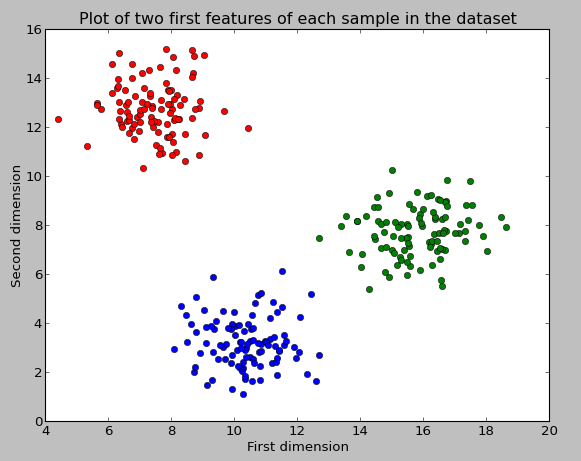
\includegraphics[width=0.4\textwidth]{img/clusteredData1.png}
    \label{fig:clusteredData1}
    \caption{Conjunto de datos con distribución normal}
\end{figure}
Ya que, a través de las RBFNN, obtenemos un modelo con la forma $f(x)=\sum w_{i}\phi(r)$ (que es caracterizado con funciones de base radial) podemos aproximar funciones complejas cuya salida sigue una distribución gaussiana (la más frecuente con mucha diferencia de entre las variables aleatorias que se dan en la naturaleza) con notable precisión. 
La figura \ref{fig:clusteredData1} es un ejemplo de datos generados con el generador de datos clusterizados que he implementado. Este recibe como parámetros básicos el número de centroides y el número de muestras y genera estos datos de forma aleatoria tomando como centro los k-centroides también tomados aleatoriamente. En las siguientes líneas introduciré esta clase sin entrar en excesivo detalle de la implementación pero sí tratando de aclarar las cuestiones que considero claves.

\subsubsection{Generación de datos aleatorios}
Para este tipo de test necesitamos generar datos que se distribuyan de forma normal alrededor de un centroide. Una distribución normal es aquella que cuya función de densidad de probabilidad queda definida por la media ($\mu$) y la desviación estándar ($\sigma$) del conjunto de datos ($x$) de la siguiente forma:
\begin{center}
$pdf(x,\mu,\sigma) = \frac{1}{ \sigma \sqrt{2 \pi}} e^{\left(-\frac{{\left(\mu - x\right)}^{2}}{2 \, \sigma^{2}}\right)}$
\end{center} 
Existen multitud de generadores aleatorios de este tipo de datos. En este caso utilizaré el propio de NumPy como muestro a continuación para generar las $n$ muestras por cada centroide ya que este definirá la media. La desviación estándard será proporcionada como parámetro en el constructor de la clase y nos permitirá jugar con la forma que adoptarán los datos generados.

\begin{figure}[!h]{}
    \centering
    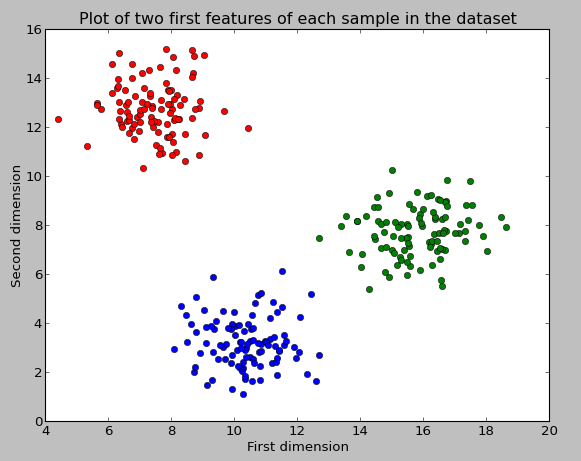
\includegraphics[width=0.4\textwidth]{img/clusteredData1.png}
    \label{fig:clusteredData1}
    \caption{Conjunto de datos con distribución normal}
\end{figure}
\section{Implementación básica de una RBF}

\section{Extendemos con centróides K-NN}

\section{PyBrain}


\chapter{Resultados}
\subsection{Pruebas de clasificación}
Ya hemos comentado anteriormente como he desarrollado el generador de datos aleatorios y como este evalúa el error del clasificador. En este proceso de evaluación consideraré una serie de conjuntos de datos con diferentes números de categorías que siguen una distribución normal en un número arbitrario de dimensiones. Sobre cada uno de estos conjuntos de datos evaluaré el funcionamiento de las distintan RBFNN estudiadas con diferente número de clústeres (neuronas con activación en base a una función de base radial en la primera capa de la red) evaluando tanto la clasificación (aciertos, fallos, falsos positivos, falsos negativos, preción y "recall") como los tiempos de entrenamiento.

\section{Comparativa de RBFNN con y sin metaplasticidad}
\section{Otros resultados de interés}



\end{document}
